\documentclass[14pt]{extbook}
\usepackage{multicol, enumerate, enumitem, hyperref, color, soul, setspace, parskip, fancyhdr} %General Packages
\usepackage{amssymb, amsthm, amsmath, bbm, latexsym, units, mathtools} %Math Packages
\everymath{\displaystyle} %All math in Display Style
% Packages with additional options
\usepackage[headsep=0.5cm,headheight=12pt, left=1 in,right= 1 in,top= 1 in,bottom= 1 in]{geometry}
\usepackage[usenames,dvipsnames]{xcolor}
\usepackage{dashrule}  % Package to use the command below to create lines between items
\newcommand{\litem}[1]{\item#1\hspace*{-1cm}\rule{\textwidth}{0.4pt}}
\pagestyle{fancy}
\lhead{Progress Quiz 5}
\chead{}
\rhead{Version B}
\lfoot{9912-2038}
\cfoot{}
\rfoot{Spring 2021}
\begin{document}

\begin{enumerate}
\litem{
Solve the linear equation below. Then, choose the interval that contains the solution.\[ \frac{8x -7}{5} - \frac{6x -5}{4} = \frac{-4x -9}{7} \]\begin{enumerate}[label=\Alph*.]
\item \( x \in [1.8, 2.1] \)
\item \( x \in [-3.5, -0.6] \)
\item \( x \in [-12, -10.3] \)
\item \( x \in [-1.6, 0.2] \)
\item \( \text{There are no real solutions.} \)

\end{enumerate} }
\litem{
Write the equation of the line in the graph below in Standard form $Ax+By=C$. Then, choose the intervals that contain $A, B, \text{ and } C$.
\begin{center}
    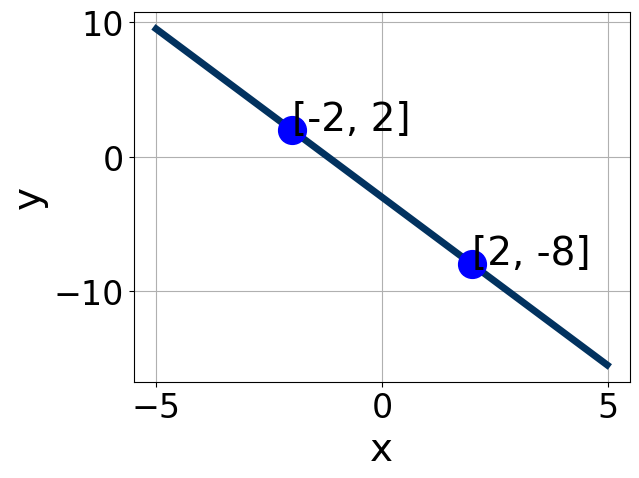
\includegraphics[width=0.5\textwidth]{../Figures/linearGraphToStandardB.png}
\end{center}
\begin{enumerate}[label=\Alph*.]
\item \( A \in [-6, -4.1], \hspace{3mm} B \in [-2.48, -1.3], \text{ and } \hspace{3mm} C \in [5.28, 6.98] \)
\item \( A \in [3, 7.5], \hspace{3mm} B \in [1.84, 2.05], \text{ and } \hspace{3mm} C \in [-6.65, -5.43] \)
\item \( A \in [2, 3], \hspace{3mm} B \in [-1.16, -0.75], \text{ and } \hspace{3mm} C \in [2.2, 3.78] \)
\item \( A \in [2, 3], \hspace{3mm} B \in [0.71, 1.27], \text{ and } \hspace{3mm} C \in [-3.09, -2.29] \)
\item \( A \in [3, 7.5], \hspace{3mm} B \in [-2.48, -1.3], \text{ and } \hspace{3mm} C \in [5.28, 6.98] \)

\end{enumerate} }
\litem{
Solve the equation below. Then, choose the interval that contains the solution.\[ -7(-2x + 18) = -16(11x + 13) \]\begin{enumerate}[label=\Alph*.]
\item \( x \in [-0.49, -0.38] \)
\item \( x \in [1.24, 2.02] \)
\item \( x \in [-2.48, -1.86] \)
\item \( x \in [-1.87, -1.67] \)
\item \( \text{There are no real solutions.} \)

\end{enumerate} }
\litem{
First, find the equation of the line containing the two points below. Then, write the equation as $ y=mx+b $ and choose the intervals that contain $m$ and $b$.\[ (11, -9) \text{ and } (-4, -7) \]\begin{enumerate}[label=\Alph*.]
\item \( m \in [0.11, 0.18] \hspace*{3mm} b \in [-6.9, -4.1] \)
\item \( m \in [-0.42, -0.11] \hspace*{3mm} b \in [-9.3, -7] \)
\item \( m \in [-0.42, -0.11] \hspace*{3mm} b \in [6.7, 10.9] \)
\item \( m \in [-0.42, -0.11] \hspace*{3mm} b \in [-5.9, -2.1] \)
\item \( m \in [-0.42, -0.11] \hspace*{3mm} b \in [-21.3, -18.8] \)

\end{enumerate} }
\litem{
First, find the equation of the line containing the two points below. Then, write the equation as $ y=mx+b $ and choose the intervals that contain $m$ and $b$.\[ (8, 11) \text{ and } (10, 5) \]\begin{enumerate}[label=\Alph*.]
\item \( m \in [-5, 0] \hspace*{3mm} b \in [-9, -2] \)
\item \( m \in [-5, 0] \hspace*{3mm} b \in [1, 6] \)
\item \( m \in [-5, 0] \hspace*{3mm} b \in [32, 38] \)
\item \( m \in [-5, 0] \hspace*{3mm} b \in [-40, -34] \)
\item \( m \in [-2, 4] \hspace*{3mm} b \in [-33, -20] \)

\end{enumerate} }
\litem{
Write the equation of the line in the graph below in Standard form $Ax+By=C$. Then, choose the intervals that contain $A, B, \text{ and } C$.
\begin{center}
    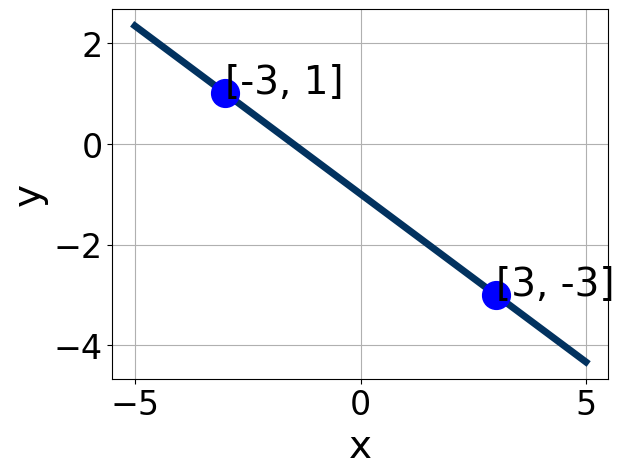
\includegraphics[width=0.5\textwidth]{../Figures/linearGraphToStandardCopyB.png}
\end{center}
\begin{enumerate}[label=\Alph*.]
\item \( A \in [-2.04, -1.15], \hspace{3mm} B \in [-4.03, -1.05], \text{ and } \hspace{3mm} C \in [2.14, 3.26] \)
\item \( A \in [0.53, 0.76], \hspace{3mm} B \in [0.64, 2.57], \text{ and } \hspace{3mm} C \in [-2.16, 0.81] \)
\item \( A \in [0.53, 0.76], \hspace{3mm} B \in [-2.59, 0.11], \text{ and } \hspace{3mm} C \in [-0.25, 1.21] \)
\item \( A \in [1.93, 2.25], \hspace{3mm} B \in [2.82, 3.97], \text{ and } \hspace{3mm} C \in [-3.64, -1.96] \)
\item \( A \in [1.93, 2.25], \hspace{3mm} B \in [-4.03, -1.05], \text{ and } \hspace{3mm} C \in [2.14, 3.26] \)

\end{enumerate} }
\litem{
Solve the equation below. Then, choose the interval that contains the solution.\[ -6(-19x + 11) = -18(2x -9) \]\begin{enumerate}[label=\Alph*.]
\item \( x \in [1.46, 2.04] \)
\item \( x \in [-0.88, -0.5] \)
\item \( x \in [0.12, 1.48] \)
\item \( x \in [-1.61, -0.72] \)
\item \( \text{There are no real solutions.} \)

\end{enumerate} }
\litem{
Find the equation of the line described below. Write the linear equation as $ y=mx+b $ and choose the intervals that contain $m$ and $b$.\[ \text{Perpendicular to } 3 x - 7 y = 12 \text{ and passing through the point } (10, 5). \]\begin{enumerate}[label=\Alph*.]
\item \( m \in [-0.87, 0.16] \hspace*{3mm} b \in [28.33, 32.33] \)
\item \( m \in [-2.67, -2.15] \hspace*{3mm} b \in [28.33, 32.33] \)
\item \( m \in [2.33, 2.75] \hspace*{3mm} b \in [-21.33, -17.33] \)
\item \( m \in [-2.67, -2.15] \hspace*{3mm} b \in [-31.33, -26.33] \)
\item \( m \in [-2.67, -2.15] \hspace*{3mm} b \in [-5, -3] \)

\end{enumerate} }
\litem{
Solve the linear equation below. Then, choose the interval that contains the solution.\[ \frac{-4x + 7}{4} - \frac{7x -6}{5} = \frac{-9x -5}{2} \]\begin{enumerate}[label=\Alph*.]
\item \( x \in [0.5, 3.1] \)
\item \( x \in [-3.6, -1.8] \)
\item \( x \in [-9.1, -8.2] \)
\item \( x \in [-2.4, -0.6] \)
\item \( \text{There are no real solutions.} \)

\end{enumerate} }
\litem{
Find the equation of the line described below. Write the linear equation as $ y=mx+b $ and choose the intervals that contain $m$ and $b$.\[ \text{Perpendicular to } 8 x + 3 y = 4 \text{ and passing through the point } (-2, 8). \]\begin{enumerate}[label=\Alph*.]
\item \( m \in [2.4, 5] \hspace*{3mm} b \in [7.77, 8.99] \)
\item \( m \in [0.2, 0.5] \hspace*{3mm} b \in [7.77, 8.99] \)
\item \( m \in [0.2, 0.5] \hspace*{3mm} b \in [9.84, 10.32] \)
\item \( m \in [-1, 0.2] \hspace*{3mm} b \in [6.63, 7.91] \)
\item \( m \in [0.2, 0.5] \hspace*{3mm} b \in [-11.7, -8.1] \)

\end{enumerate} }
\end{enumerate}

\end{document}